\section{Schraubklemme zur Versorgung des Zusatzprints}
Die Schraubklemme zur Versorgung des Zusatzprints befindet sich auf der rechten Seite des Zusatzprints (Abb. \ref{fig:Zusatzprint}).

\section{Schraubklemmen für die 4-20mA Datenleitungen}
Der Zusatzprint kann bis zu 8 Sensoren auslesen. Die Leitungen werden dazu an die beiden Schraubklemmen auf der oberen Seite des Zusatzprints (Abb. \ref{fig:Zusatzprint}) angehängt.
Standardmäßig ist der erste ADC aktiviert und der zweite ADC deaktiviert.
Wenn mehr als 4 Sensoren eingelesen werden wollen, muss der zweite ADC softwaretechnisch erst aktiviert werden.

\section{Schraubklemme zur Versorgung der Sensoren}
Eine Schreibklemme, an der 24V Gleichspannung anliegen, befindet sich neben den Schraubklemmen für die Datenleitungen (Abb. \ref{fig:Zusatzprint}) und ist dazu gedacht, die Sensoren zu versorgen.\\
Es können in eine Öffnung mehrere Kabel gesteckt werden, wenn mehr als 4 Sensoren versorgt werden sollen.

\section{Schraubklemme um die Sensoren mit GND zu verbinden}
Die Schraubklemme, um die Sensoren mit GND zu verbinden, befindet sich neben der Schraubklemme für die Versorgung der Sensoren (Abb. \ref{fig:Zusatzprint}).\\
Auch hier können mehrere Kabel in eine Öffnung gesteckt werden.

\newpage
\begin{figure}[h]
    \centering
    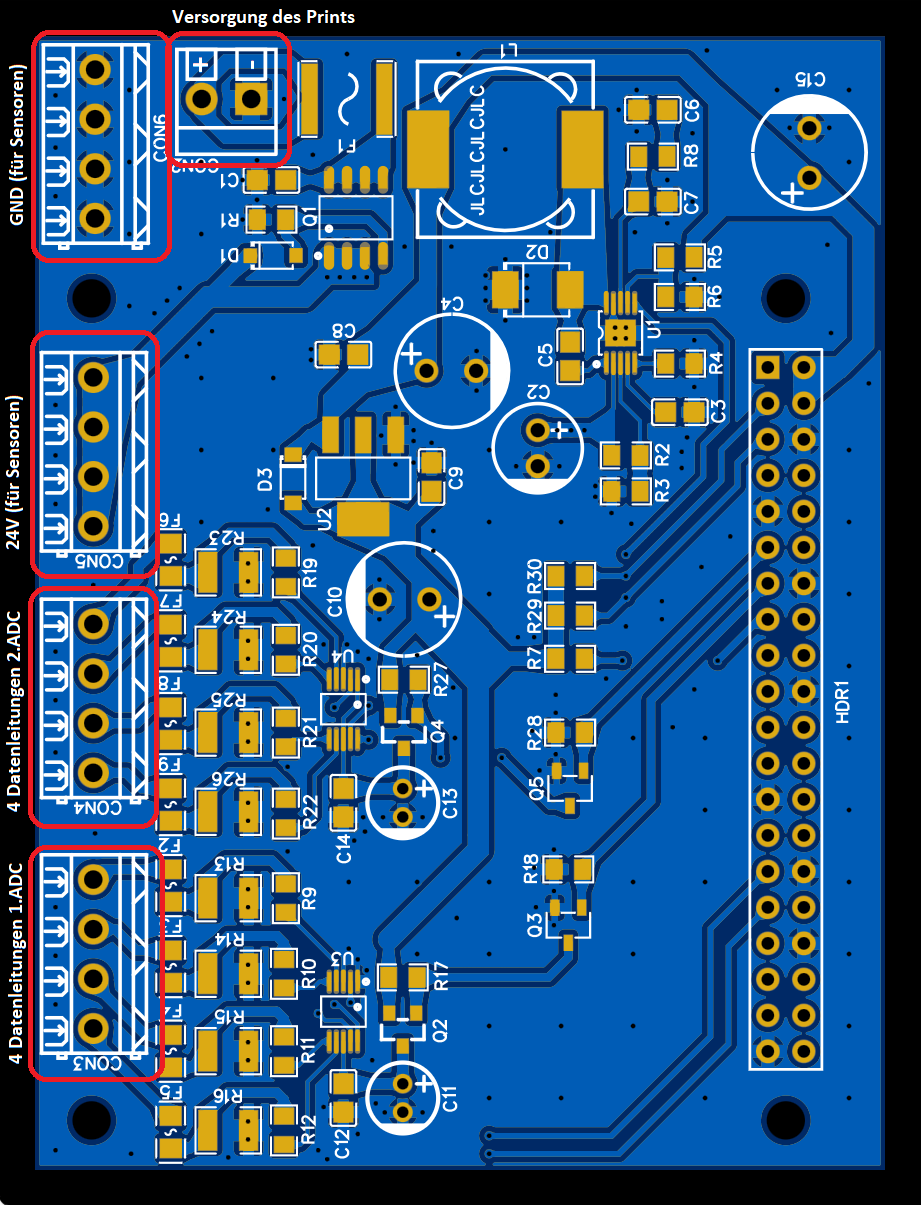
\includegraphics[width=1\linewidth]{Images/PCB1.PNG}
    \caption{Zusatzprint}
    \label{fig:Zusatzprint}
\end{figure}